%%%%%%%%%%%%%%%%%%%%%%%%%%%%%%%%%%%%%%%%%%%%%%%%%%%%%%%%%%%%%%%%%%%%%%%%%%%%%%%%
% spec.tex
% Toplevel specification of the Memory Model
%
% 
%%%%%%%%%%%%%%%%%%%%%%%%%%%%%%%%%%%%%%%%%%%%%%%%%%%%%%%%%%%%%%%%%%%%%%%%%%%%%%%%

%----------------------------------
\chapter{Product Specification}\hyperdef{part}{spec}{}
\label{ch:overview:spec}
%----------------------------------

\section{Conceptual Design}
Several factors drove the design of the \ModelDesc.

\paragraph{Environment.}
The model is to work within and outside of the Trick environment.

\paragraph{Flexibility.}
The model is to work with a wide variety of data types, including
pointers, C++ primitive types, and classes.

\paragraph{C++ Concerns.} The C++ allocation operators
\verb|new| and \verb|new[]| have distinct semantics,
as do \verb|delete| and \verb|delete[]|.
The \ModelDesc needs to provide analogous capabilities.

\paragraph{Ease of Use.} The \ModelDesc should be easy to use. Details of the
above concerns should be hidden from the programmers who use the model.

\paragraph{Backward Compatibility.} While the JEOD 2.1 \ModelDesc
represents a marked change in functionality, the extermal interfaces
to the model remain unchanged.

\paragraph{Thread Safety.} The JEOD 2.0 implementation of the model was
solely in the form of macros. Ensuring that JEOD was thread-safe fell upon the
simulation engine. Adding substance to the model required making thread safety a foremost concern in the design and implementation of the model.

\subsection{Interactions}

\subsubsection{JEOD Models Used by the \ModelDesc}
The \ModelDesc uses the following JEOD models:
\begin{itemize}
\item\hypermodelref{MESSAGE}. The \ModelDesc uses the \MESSAGE\ to report error conditions and optionally, to generate debug output.
\item\hypermodelref{NAMEDITEM}. The \ModelDesc uses the \NAMEDITEM\ to demangle the type name in a std::type\_info object.
\item\hypermodelref{SIMINTERFACE}. The \ModelDesc uses the \SIMINTERFACE\ as the mechanism via which memory allocations and deallocations are registered with
the simulation engine.
\end{itemize}

\subsubsection{Use of the \ModelDesc in JEOD}
All JEOD models that dynamically allocate memory must use the \ModelDesc for
those allocations if the allocated memory needs to be visible to the simulation
engine for any reason (user input, logging, checkpoint/restart, \ldots).
Most JEOD models use the \ModelDesc because of this mandate.

\subsection{Macros}
The primary external interface to the model are the \ModelDesc macros intended
for external use. The signatures (names and arguments) of these macros
remain unchanged from JEOD 2.0. The implementations of these macros differs
significantly from JEOD 2.0.

The bodies of the external macros expand into invocations of \ModelDesc macros
intended for internal use only. Because these internal macros are clearly
designated as such, the arguments and even the names of these internal macros
do differ from their JEOD 2.0 counterparts.
In JEOD 2.1, these internal macros expand into creation of \ModelDesc objects
and calls to \ModelDesc member functions.

\subsection{Classes}
The \ModelDesc comprises several classes and templates.
The JeodMemoryManager class is a singleton class that
allocates, keeps track of, and deallocates memory.
The manager keeps track of allocated memory and data types.
The manager represents each block of allocated memory as an instance of
the JeodMemoryItem class.
Instances of template classes that derive from the
JeodMemoryTypeDescriptor class represent data types. Each unique
data type is represented by a different generated class.

\subsubsection{JeodMemoryManager}
The JeodMemoryManager class provides the interface between the \ModelDesc
macros and the rest of the JEOD memory model.
All nonstatic member functions and all member data are private.
The public interface is via the publicly visible static member functions.
Each public static member function relays the method call to the singleton
memory manager via a correspondingly-named private member function.

\paragraph{Singleton.}
The class is intended to be a singleton. The constructor ensures that at most
one instance of the class exists. The publicly visible static member functions
ensure that an instance of the class does exist.
Each public static member function invokes a correspondingly-named private
non-static member function on this singleton instance.

\paragraph{Maps.}
The memory manager uses map and table objects
to track extant allocated memory,
to store information about the types of data that have been allocated,
and to store information about where in the code those allocations occurred.

\paragraph{Thread Safety.}
The maps and tables, along with other data members of the class, must be
accessed and updated in a thread-safe manner.
To ensure the constraint is satisfied, access to these elements is
protected by means of a mutex and is limited to a small number of
member functions.
Thread safety is further ensured by encoding these potentially unsafe
member functions in a systematic way.

\subsubsection{JeodMemoryItem}
The model uses the JeodMemoryItem class to represent blocks of allocated memory.
Each block of allocated memory is represented by an instance of this class.
The memory manager maintains an STL map that maps the address of a memory block
to the JeodMemoryItem object that describes that block.
A JeodMemoryItem object contains information about the size and type of
an allocated block of memory. It also contains a unique identifier that will
eventually be used when checkpoint/restart capabilities are added to the model.

\subsubsection{JeodMemoryTable}
One challenge with recording information about each allocated block of memory
is that using 64 bit addresses can make for rather high overhead.
A JeodMemoryItem object occupies only 16 bytes in part due to the use of
classes that derived from JeodMemoryTable. A memory table indirectly maps keys
to values. A memory table comprises an STL map and an STL vector of values.
The STL map object maps keys to index numbers into the vector. A JeodMemoryItem
object stores index numbers rather than keys, resulting in a significant
reduction in overhead on a 64 bit machine.
 
\subsubsection{JeodMemoryTypeDescriptor}
The model uses the JeodMemoryTypeDescriptor class to represent data types.
The class JeodMemoryTypeDescriptor is a pure virtual class.
Two template classes derive from this base class,
one for non-structured data and the other for structured data.
Each data type is represented by an instance of a class generated from one
of these two template classes.
A JeodMemoryTypeDescriptor contains information about
the size of an instance of the data type represented by the type descriptor
and the name of the type. Key member functions of the class address the issue of
deleting and destroying allocated memory and the issue of determining whether
a pointer to some interior address is in fact a base class pointer.

\subsection{Simulation Assumptions and Limitations}
\label{sec:contraints}
This model places certain limitations on the architecture of a JEOD-based
simulation.
\begin{enumerate}
\item The JeodMemoryManager destructor uses the simulation's message handler
  to report errors discovered during destruction and may eventually use
  the simulation's simulation engine memory interface to revoke the
  registration of memory allocated by JEOD that has not been freed.
  This in turn means that:
  \begin{enumerate}
  \item The simulation's message handler and simulation engine memory
    interface must be destructed after destructing the memory manager.
  \item The destructors for those objects cannot use the memory manager.
  \end{enumerate}
\item The JEOD memory allocation and deallocation macros expand into calls
  to memory manager member functions. The memory manager must be viable
  (constructed and not yet destructed) for these calls to function properly.
  This in turn means that the memory manager must be constructed very
  early in the overall construction process and destructed very late in
  the overall destruction process.
\item The supported solution to both of these issues is to use a compliant
  derived class of the JeodSimulationInterface class and to ensure that
  this composite object is created early and destroyed late. In a Trick-07
  simulation, this can be accomplished simply by placing a declaration of
  an object of type JeodTrickSimInterface near the top of an \Sdefine file.
  The recommended placement is just after the Trick system sim object.
\end{enumerate}

This model also makes certain assumptions regarding the behavior of the
simulation engine.
\begin{enumerate}
\item The simulation engine will not spawn threads that use the \ModelDesc
  to allocate memory until after the JeodSimulationInterface object
  that contains the memory manager object has been constructed.
\item The simulation engine will join all threads that use the \ModelDesc
  prior to destroying the JeodSimulationInterface object.
\end{enumerate}
The Trick-07 simulation engine satisfies these assumptions given a simulation
built according to the above limitations.

\section{Mathematical Formulations}
N/A

\section{Detailed Design}
\label{sec:detailed_design}

\subsection{\ModelDesc Macros}
\label{sec:macros}
The primary external interface to the model is in the form of macros
that are explicitly marked as externally-usable. These in turn expand into
invocations of internal macros. The internal macros in turn expand into
calls to JeodMemoryManager static member functions.

Tables~\ref{tab:ext_macros}and ~\ref{tab:primitives} list the externally-usable and the underlying primitive JEOD memory management macros.
See the model API documentation for details.

\begin{table}[htp]
\centering
\caption{Externally-Usable \ModelDesc Macros}
\label{tab:ext_macros}
\vspace{1ex}
\begin{tabular}{||l|l|} \hline
{\bf Macro} & {\bf Description} \\ \hline \hline
\verb|JEOD_ALLOC_CLASS_MULTI_POINTER_ARRAY| & Allocate array of pointers \\
\verb|JEOD_ALLOC_CLASS_POINTER_ARRAY|       & Allocate array of pointers \\
\verb|JEOD_ALLOC_CLASS_ARRAY|               & Allocate array of objects \\
\verb|JEOD_ALLOC_PRIM_ARRAY|                & Allocate array of primitives \\
\verb|JEOD_ALLOC_CLASS_OBJECT|              & Allocate one structured object \\
\verb|JEOD_ALLOC_PRIM_OBJECT|               & Allocate one primitive object \\
\verb|JEOD_STRDUP|                          & Duplicate a string \\
\verb|JEOD_IS_ALLOCATED|                    & Was memory allocated by this model? \\
\verb|JEOD_DELETE_ARRAY|                    & Delete array of pointers \\
\verb|JEOD_DELETE_OBJECT|                   & Delete allocated object \\
\hline
\end{tabular}
\end{table}

\begin{table}[htp]
\centering
\caption{Primitive Macros}
\label{tab:primitives}
\vspace{1ex}
\begin{tabular}{||l|l|} \hline
{\bf Macro} & {\bf Description} \\ \hline \hline
\verb|JEOD_MEMORY_DEBUG_INTERNAL|  & Debug level cast to enum value \\
\verb|JEOD_ALLOC_OBJECT_FILL|      & Fill pattern for structured types \\
\verb|JEOD_ALLOC_PRIMITIVE_FILL|   & Fill pattern for primitive types \\
\verb|JEOD_ALLOC_POINTER_FILL|     & Fill pattern for pointer types \\
\verb|JEOD_ALLOC_TYPE_IDENTIFIER|  & Allocate type identifier for a type \\
\verb|JEOD_ALLOC_CLASS_IDENTIFIER| & Allocate class identifier for a type \\
\verb|JEOD_ALLOC_CREATE_MEMORY|    & Allocate and register memory \\
\verb|JEOD_ALLOC_ARRAY_INTERNAL|   & Allocate an array of objects \\
\verb|JEOD_ALLOC_OBJECT_INTERNAL|  & Allocate a single instance \\
\verb|JEOD_DELETE_INTERNAL|        & Delete memory \\
\hline
\end{tabular}
\end{table}

\subsection{JeodMemoryManager}
\subsubsection{Public Interface}
The public interface to the memory manager is in the form of static member
functions. These static member functions test whether the singleton memory
manager instance exists, and if it does, operates on that method. 

\subsubsection{Thread Safety}
Thread safety was a major concern in the design and implementation of the model.
The following JeodMemoryManager data members could become corrupted in a
multi-threaded environment without adequate protection:
\begin{itemize}
\item \verb|alloc_table| - Maps memory addresses to memory items.
\item \verb|type_table| - Maps RTTI names to type descriptors.
\item \verb|string_table| - Maps unique strings to themselves.
\item \verb|cur_data_size| - Current size of allocated data.
\item \verb|max_data_size| - Maximum of the above.
\item \verb|max_table_size| - Maximum allocation table size.
\item \verb|allocation_number| - Number of allocations made.
\end{itemize}

Several precautions are taken to protect against such corruption.
Access to these protected data is limited to three groups of member functions.
\begin{enumerate}
\item The non-default constructor, the destructor, and member functions
  called only by the constructor and destructor (\verb|generate_shutdown_report|
  in the current implementation).
  These member functions have free access to the protected data.
  This unfettered access will not result in corrupted data if the simulation 
  and the simulation engine are constructed and behave according to the
  assumptions and limitations specified in section~\ref{sec:contraints}.
\item Methods whose names end in \verb|_atomic|. These member functions use the
  mutex lock and unlock member functions (see
  section~\ref{sec:exclusive_access}) to ensure exclusive access to
  sensitive data. Calls to other JeodMemoryManager member functions by
  members of this group of member functions are limited to the mutex lock and
  unlock member functions and the \verb|_nolock| methods (next group), with the
  latter only called within a protected block of code. These \verb|_atomic|
  member functions must not and do not call one another as doing so would lead
  to either a lock error or deadlock.
\item Methods whose names end in \verb|_nolock|. These member functions also
  have unfettered access to the sensitive data. Members of either of the two
  previous groups can call these member functions. Currently there is only one
  such member function, \verb|get_type_descriptor_nolock|.
\end{enumerate}

Figure~\ref{fig:protected_data_access} depicts the access to the protected data by the \verb|_atomic| member functions. The figure also depicts the
member functions that directly or indirectly call these atomic member functions.
Member functions are depicted as ovals,
member data as parallelograms,
function calls as solid lines, and
data access as dashed lines.

\begin{figure}[hbtp]
\centering
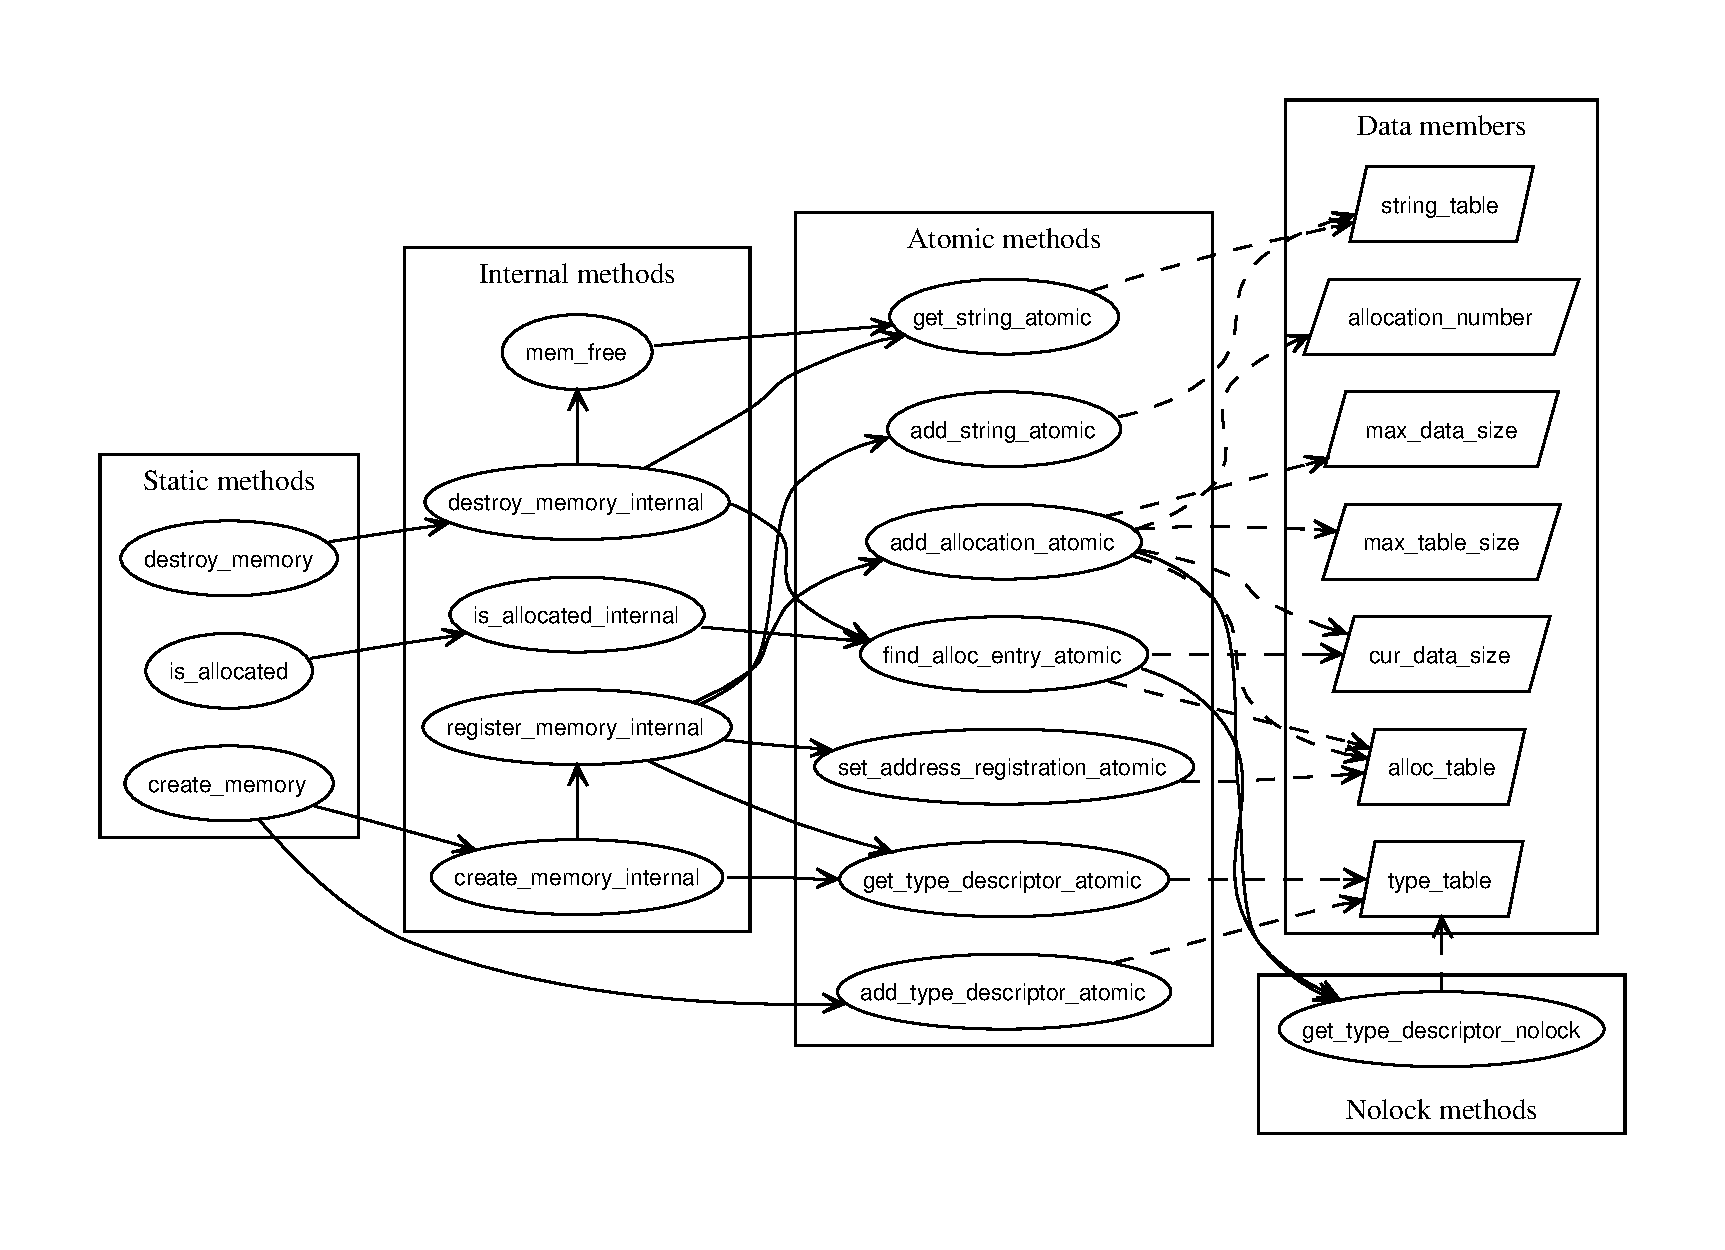
\includegraphics[width=6.5in]{atomic_methods}
\caption{Protection of Thread-Sensitive Data}
\label{fig:protected_data_access}
\end{figure}

\subsubsection{Exclusive Access}\label{sec:exclusive_access}
The JeodMemoryManager contains a POSIX mutex data member whose purpose is to
ensure exclusive access to the data that could otherwise become corrupted in a
multi-threaded environment. The mutex is created by the constructor and
destroyed by the destructor. (This is another reason for the constraints on the
simulation architecture and the simulation engine.)

Only two other member functions directly access this mutex. These are the
\verb|begin_atomic_block| and \verb|end_atomic_block| member functions.
The former function obtains a lock on the mutex, preventing any other thread
from becoming active until the lock is released.
The latter function releases the lock, once again allowing the system to switch
threads to optimize performance. One key finding of the model peer review
was that these methods should nominally return only if the request was
successful. Failure to obtain or release the lock constitutes a fatal error.
This simplifies the design of the functions themselves and that of the
calling functions.
The function \verb|begin_atomic_block| obeys this dictum strictly.
The function \verb|end_atomic_block| takes an argument that indicates
whether it should or should not ignore errors. When the argument is false
(nominal usage) \verb|end_atomic_block| checks for errors and returns only
if the lock is successfully released. When the argument is true the function
attempts to release the lock but does not check the status of the request.
Calling functions use this latter capability when a fatal error has already
been detected.

The only member functions that call
\verb|begin_atomic_block| and \verb|end_atomic_block| are the
\verb|_atomic| functions. All of the \verb|_atomic| member functions are
written as follows:
\begin{verbatim}
   try {
      begin_atomic_block ();
      // Operate on member data at will
      if (<error_condition>) {
         end_atomic_block (true);
         MessageHandler::fail (...);
         return;
      }
      // Continue operating on member data at will
      end_atomic_block (false);
   }
   catch (...) {
      end_atomic_block (true);
      throw;
   }
\end{verbatim}


\section{Waivers}
The data member \verb|JeodMemoryManager::mutex| is \verb|mutable|, a forbidden
word per the JEOD coding standards. The coding standards allow for waivers to
the standards if the exception is justified. This section provides the
explanation needed to enable the use of that word in this case.

The \verb|mutable| keyword tells the compiler to ignore modifications to
mutable elements in an otherwise \verb|const| method.
The \verb|mutex| data member is qualified as being mutable because,
athough its value does change with a successful lock, it is restored
to its prelock value with an unlock. A method that could otherwise qualify
as a \verb|const| method can still be a const method by marking the mutex
as mutable. Mutexes are one of the well-accepted types of data that typically
are designated as mutable.

\newpage
\section{Inventory}
All \ModelDesc files are located in the directory
{\tt \$\{JEOD\_HOME\}/models/utils/memory}.
Relative to this directory,
\begin{itemize}
\vspace{-0.2\baselineskip}
\item Header and source files are located
in the model {\tt include} and {\tt src} subdirectories.
Table~\ref{tab:source_files} lists the 
configuration-managed files in these directories.
\vspace{-0.1\baselineskip}
\item Verification files are located in the model {\tt verif} subdirectory.
See table~\ref{tab:verification_files}
for a listing of the 
configuration-managed files in this directory.
\vspace{-0.1\baselineskip}
\item Documentation files are located in the model {\tt docs} subdirectory.
See table~\ref{tab:documentation_files}
for a listing of the 
configuration-managed files in this directory.
\end{itemize}

\input{inventory}
